\chapter{Marco teórico}
\label{ch:marco-teorico}

En 1975 John Holland propone imitar los procesos biológicos naturales que rigen la selección natural usando ordenadores, lo que sería el principio de los \glspl{ag}~\cite{holland1975}. En un AG, las soluciones son modeladas como individuos o cromosomas, que generalmente se representan como cadenas de bits, aunque también se puede usar otro tipo de cadenas. Estas soluciones son evaluadas por una función de aptitud o fitness, y las más adecuadas son selecciondas para reproducirse mediante cruzamiento y mutación, procesos que mezclan y alteran aleatoriamente los cromosomas para generar diversidad. Los descendientes resultantes forman nuevas generaciones que vuelven a ser evaluadas, creando un ciclo que se repite hasta cumplir alguna condición de parada, como pudiera ser un número limitado de generaciones o que se alcance la solución deseada.

\begin{figure}[H]
    \centering
    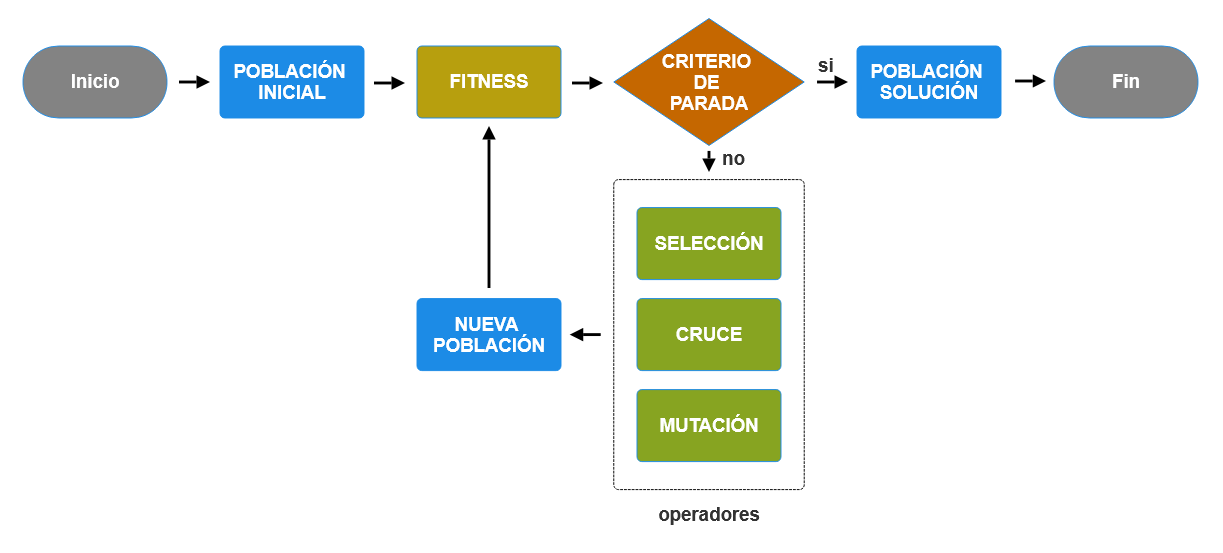
\includegraphics[width=1\textwidth]{figures/algoritmo-genetico.png}
    \caption{Algoritmo genético simple.}
    \label{fig:algoritmo-genetico}
  \end{figure}

Explicado el concepto general, se va a desglosar cada una de las fases de la figura \ref{fig:algoritmo-genetico}, que muestra el esquema básico de un algoritmo genético.

\section{Población}

Antes de explicar la generación de una población inicial, es necesario conocer algunos conceptos que son usados para representar y entender las soluciones. Son términos que son usados en la biología y en el campo de la genética. 

\begin{itemize}
    \item \textbf{Gen.} Es la unidad básica de información en un cromosoma. En una cadena de bits que representa una solución, cada bit puede considerarse un gen. En el caso que se trata en este PFG, el menú semanal, cada tipo de comida se podría considerar un gen. Por ejemplo, un gen sería bebida, plato principal o postre.
    \item \textbf{Alelo.} Es la forma específica o valor que puede tomar un gen. Siguiendo el ejemplo de bebida, posibles alelos serían agua, té o cerveza.
    \item \textbf{Cromosoma.} Es una colección de genes y representa una solución completa al problema de optimización. El cromosoma es la cadena de bits completa. En nuestro caso, la lista completa de alimentos seleccionados para una semana es el cromosoma. 
    \item \textbf{Fenotipo.} Es la manifestación real de la solución codificada. En el PFG sería cómo se preparan y sirven estos alimentos en la realidad.
\end{itemize}

En la figura \ref{fig:cromosoma} se expone la estructura de un cromosoma con el ejemplo del menú semanal de comida.

\begin{figure}[H]
  \centering
  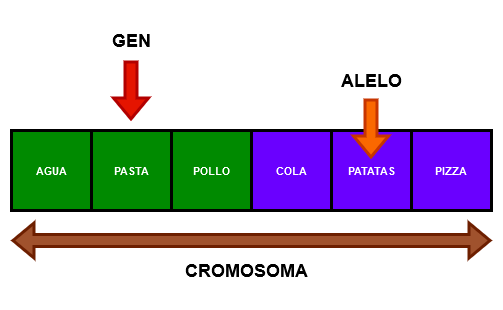
\includegraphics[width=0.625\textwidth]{figures/cromosoma.png}
  \caption{Estructura de un cromosoma.}
  \label{fig:cromosoma}
\end{figure}

La generación de una población inicial implica crear un conjunto de soluciones candidatas. Generalmente, los individuos son seleccionados aleatoriamente dentro de los límites definidos en cada problema, asegurando que todas las áreas del espacio de búsqueda puedan ser exploradas. También existen métodos alternativos de generación que aplican ciertas restricciones para formar soluciones iniciales más prometedoras. Tomando de ejemplo el menú semanal, el espacio de búsqueda comprendería la base de datos en la que aparecen todos los alimentos con sus respectivas calorias y macronutrientes. 

\section{Evaluación}

Se mide lo bueno que es un individuo para nuestros propósitos (la calidad del individuo). Lo más importante es definir una función de fitness correcta y representativa del problema a evaluar. Si se trata de un problema multiobjetivo, se tendrá que diseñar una función de fitness diferente por cada objetivo.

Según vayan pasando generaciones, la población inicial irá evolucionando hacia poblaciones candidatas que presentarán una mejor aptitud. Si la población ha alcanzado el objetivo, la condición de parada se activará, convirtiendo el conjunto de individuos candidatos en la población solución. En caso de no alcanzarlo, seguirá evolucionando hacia otra población candidata distinta.

Para diseñar una función de fitness acorde al problema y al objetivo (u objetivos) se pueden seguir los siguientes pasos:

\begin{enumerate}
  \item Determinar si el objetivo es maximizar o minimizar un valor específico. En el caso que se trata en este proyecto, se busca que la diferencia entre las calorias necesarias y la suma de las calorias de los alimentos sea la menor posible, por lo que se trataría de un problema de minimización.
  \item Identificar las restricciones. En el ejemplo, una podría ser los límites superior e inferior de calorías permitidas.
  \item Definir la función matemática que represente el objetivo del problema. Si existen múltiples objetivos, se pueden ponderar.
  \item Incorporar las penalizaciones para soluciones que no cumplan con las restricciones.
\end{enumerate}

Por lo tanto, la mejor solución debería recibir la mejor evaluación. Esto ayudará al algoritmo a entender el camino a seguir, ya que penalizará las soluciones infactibles.

\subsection{Restricciones}

Uno de los apartados a destacar cuando se diseña la función de calidad es entender cómo se manejan las restricciones para asegurar que las soluciones generadas sean viables y de alta calidad.

Existen tres tipos de restricciones que limitan el espacio de soluciones válidas. Sea \textit{x} las variables del problema:

\begin{itemize}
  \item Restricciones de igualdad. $h_j(x) = 0$
  \item Restricciones de desigualdad. $g_k(x) \geq 0$ ó $g_k(x) \leq 0$
  \item Restricciones de contorno o de caja (\textit{box-constraints}). $x^L \leq x \leq x^U$
\end{itemize}

Estos tipos de restricciones se pueden tratar mediante distintos métodos.

\begin{itemize}
  \item \textbf{Funciones de penalización.} Se penalizan las soluciones infactibles. Estas penalizaciones representan cómo de lejos está la solución de la región factible.
  \item \textbf{Separatista.} Dividen el problema en subproblemas más manejables que se pueden resolver por separado y luego combinar.
  \item \textbf{Preservación de la factibilidad.} Se usan representaciones especiales (codificación binaria, entera, real, etc.) que simplifican la forma del espacio de búsqueda y operadores que mantienen la factibilidad de las soluciones, lo que elimina las soluciones inválidas en cada etapa del algoritmo.
  \item \textbf{Reparación.} Se modifican las soluciones candidatas infactibles de forma que no violen las restricciones.
\end{itemize}

\subsection{Condición de parada}

Como se ha mencionado, tras la evaluación de calidad la condición de parada determina cuándo el algoritmo debe detenerse y presentar la solución. Si bien existen una gran variedad de condiciones de parada, las más comunes son:

\begin{itemize}
  \item Aptitud del individuo. El algoritmo se detiene si se alcanza una solución, ya sea alcanzando el valor objetivo o estando dentro de unos umbrales predefinidos.
  \item Número máximo de generaciones. Se para si la población ya ha evolucionado un número de veces predefinido.
  \item Tiempo máximo de ejecución. Parecida a la anterior, pero con un tiempo máximo.
  \item Convergencia. Se puede detener la ejecución si la población muestra poca o ninguna mejora en la aptitud durante un número determinado de generaciones consecutivas.
\end{itemize}

\section{Operadores}

Son los procesos que se aplican a poblaciones de individuos para desarrollar generaciones futuras. Sirven para la exploración del espacio de soluciones y para la mejora de las poblaciones a través de las generaciones. Se busca que el conjunto de individuos presente una alta diversidad, ya que si es baja se corre el riego de caer en mínimos locales, lo que no permitiría explorar el espacio de soluciones ampliamente. En la figura \ref{fig:operadores} aparecen los operadores básicos en los algoritmos evolutivos, que son los que se van a explicar en más detalle.

\begin{figure}[H]
  \centering
  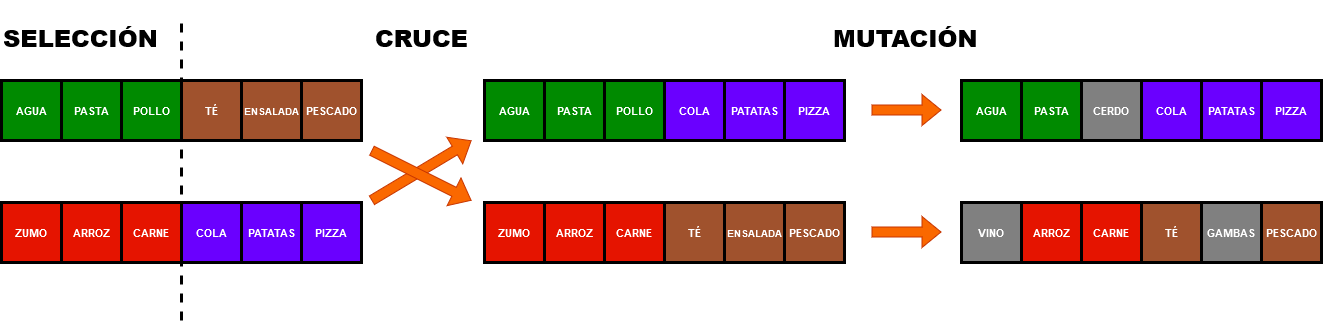
\includegraphics[width=1\textwidth]{figures/operadores.png}
  \caption{Operadores.}
  \label{fig:operadores}
\end{figure}

\subsection{Selección}
\label{Seleccion}

El primero de los operadores básicos. Elige un individuo para reproducirlo. Comúnmente, se busca un equilibrio entre la diversidad y la convegencia. El algoritmo debe explorar el espacio de búsqueda en amplitud, ya que podría caer en mínimos locales si la población es muy parecida entre sí, lo que no permitiría encontrar buenas soluciones. Pero también es de interés que las poblaciones candidatas vayan evolucionando hacia una mayor aptitud, reconduciendo el algoritmo por zonas del espacio de búsqueda más probables de encontrar una solución.

Si bien se puede seleccionar de manera equiprobable, existen métodos basados en la aptitud del individuo que buscan respetar este equilibrio. Estos son algunos:

\begin{itemize}
  \item \textbf{Método estándar (rueda de la fortuna).} Asigna a cada individuo una probabilidad proporcional a su fitness, por lo que los más aptos tienen mayor probabilidad de reproducirse. Existe un derivado de este método en el que se normalizan las probabilidades, lo que favorece aún más a los adaptados.
  \item \textbf{Método del rango.} Se ordenan los individuos según su aptitud, y la probabilidad de selección se asigna según este ránking.
  \item \textbf{Selección por torneo.} Se escoge aleatoriamente un subconjunto de individuos de la población, y el mejor de este es elegido.
\end{itemize}

\subsubsection{Selección ambiental (Remplazo)}

A parte de los métodos basados en la aptitud, se puede usar usa la técnica de la selección ambiental para seleccionar aquellos individuos que puedan influir significativamente en la eficacia del algoritmo genético. Existen varios métodos de selección ambiental:

\begin{itemize}
  \item \textbf{Reemplazo generacional completo.} Método tradicional en la selección y explicado en el apartado \ref{Seleccion}. Toda la población actual es reemplazada por una nueva. Promueve altas tasas de diversidad, pero conlleva una aptitud de los individuos irregular.
  \item \textbf{Reemplazo generacional parcial (\textit{Steady-State}).} Solo una parte de la población es reemplazada en cada generación. Se promueve una mejora constante en la calidad ya que las soluciones con un fitness elevado pueden mantenerse.
  \item \textbf{Reemplazo elitista.} Escoge los mejores individuos de una generación para que se mantengan en la siguiente. Esto ayuda a que la calidad del mejor individuo de una generación sea siempre igual o superior a su equivalente de la generación anterior, consiguiendo una progresión constante hacia la solución óptima, es decir, una mayor convergencia.
  \item \textbf{Selección $(\mu,\lambda)$.} De $\mu$ padres se generan $\lambda$ hijos. Los $\mu$ mejores de los $\lambda$ hijos forman la siguiente generación de padres.
  \item \textbf{Selección $(\mu+\lambda)$.} Igual que en la anterior, de $\mu$ padres se generan $\lambda$ hijos, pero en este caso los $\mu$ mejores de la combinación entre los $\mu$ padres y los $\lambda$ hijos forman la siguiente generación.
\end{itemize}

\subsection{Cruce}

Se combina el material genético de dos individuos, padres, para producir descendencia, hijos. Es decir, se utiliza para intercambiar características de dos soluciones parentales con el objetivo de generar nuevas soluciones. Se aplica con probabilidad \(P_c\) . Al promover la mezcla de genes, ayuda a aumentar la diversidad y la convergencia, debido a la generación de nuevos descendientes con características deseables. Se usan distintos métodos:

\begin{itemize}
  \item \textbf{Cruce de un punto.} Como se muestra en la figura \ref{fig:cruce}, se selecciona aleatoriamente una posición en el cromosoma. Todos los genes que están antes de este punto se intercambian con los que están después en la otra cadena, y viceversa, para producir dos nuevos descendientes.
  
  \begin{figure}[H]
    \centering
    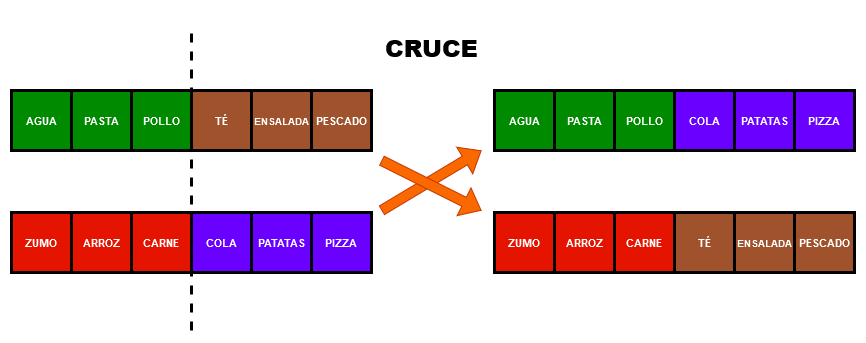
\includegraphics[width=1\textwidth]{figures/cruce.png}
    \caption{Cruce de un punto.}
    \label{fig:cruce}
  \end{figure}

  \item \textbf{Cruce de dos puntos.} Similar al cruce de un punto, pero se seleccionan dos puntos de corte. Las cadenas de genes entre estos dos puntos se intercambian entre los dos padres.
  \item \textbf{Cruce uniforme.} Cada gen tiene una probabilidad igual de ser elegido de uno de los dos padres.
\end{itemize}

\subsection{Mutación}

Último de los operadores básicos. Se recorre toda la cadena, mutando cada gen con probabilidad \(P_m\) , es decir, eligiendo un nuevo valor mediante una elección equiprobable sobre el alfabeto. La mutación aumenta la diversidad y ayuda a no caer en mínimos locales. Algunos de los métodos usados son:

\begin{itemize}
  \item \textbf{Mutación uniforme.} Cada gen puede cambiar a otro valor con probabilidad \(P_m\) , como se expone en la figura \ref{fig:mutación}.

  \begin{figure}[H]
    \centering
    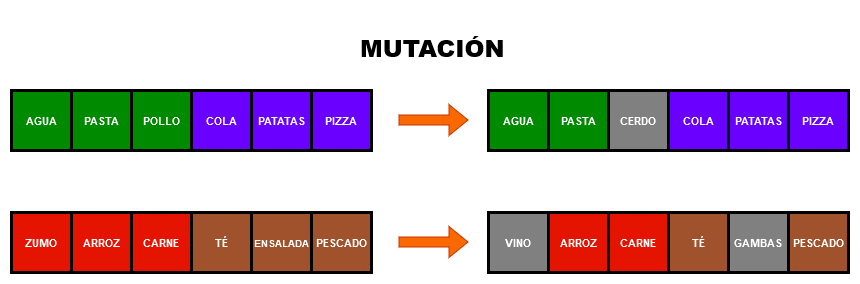
\includegraphics[width=1\textwidth]{figures/mutacion.png}
    \caption{Mutación uniforme.}
    \label{fig:mutación}
  \end{figure}

  \item \textbf{Mutación por intercambio.} Dos genes aleatorios en el cromosoma son seleccionados y sus posiciones se intercambian. 
\end{itemize}

